
{\chapter{Exploring the single-cell RNAseq analysis landscape in timeseries patient derived xenografts}

}
 \label{ch:Chapter5}
 \section{Motivation}

In spite of advanced technologies and treatment, triple negative breast cancer still facing the problems of tumor recurrence and drug resistance.
For any given difference between the types of drug resistance, for example, the expression of a particular gene, it is assumed that differences arise deterministically or probabilistically in the configuration of transcription factors regulating the genes in the tumors. Cancer cells in distinct cell- states often exhibit important differences in functional properties depending on the which genes are turned on and off resulting in sensitive or resistant phenotype.

The most challenging analysis is to differentiate whether the change in gene expression leading to change in cellular state is stochastic\cite{raj2008nature} and random or its deterministic to produce the same output under similar environment.
Cancer cells in distinct cell- states often exhibit important differences in functional properties depending on which genes are turned on and off resulting in sensitive  or resistant phenotype.
Previously it is shown that unique cells within a population can exhibit fluctuations in expression of a group of genes, that could predict distinct phenotypes \cite{shaffer2019memory}.

Un-like genomic clones that could get selected in resistant phenotype \cite{salehi2020single}, we still are not clear whether the cell-states are acquainted for this kind of behaviour or the selected states are pre-existing in the cancer population and under continuous pressure shows obvious dynamics or there is a transition from one state to another that ultimately gets selected over time. Because of difficulty to analyse longitudinal patient's samples for single cell gene expression and lack of multiple longitudinal pre-clinical breast cancer models, these questions remains unexplored. Our understanding of these processes, and how they relate to triple negative breast cancer heterogeneity, is limited.
Here we set to explore timeseries three breast cancer patient derived xenografts (PDX) that were serially challenged for around 4-5 cycles with the drug until they started showing less response to the treatment.The aim is to measure the magnitude of fluctuations in gene expression from sensitive to resistant phenotype.


 \section{Synopsis}
 From the previous chapter we know that the population changes with the tumor growth from one passage to another with and without the drugs. We see the shifts in the clones and some clones get selected and others disappear.
For this chapter, to explore the cellular compositions and heterogeneity under diverse conditions, in breast cancer, we performed scRNAseq analysis on the same 3 patient derived xenograft timeseries tumors used as substrates in chapter 4. We acquired transcriptional signatures comprising of total of 171,560 individual cells including -------cells from untreated tumors, ----------cells from cisplatin treated tumors, ----------cells from cisplatin drug holiday tumors, ---------cells from CX-5461 treated tumors and -----------cells from CX-5461 drug holiday tumors.
 
In order to pursue our analysis in single cell RNA space, first, we summarized the clonal identities from chapter 4 into sensitive and resistant. We assume that the clones that show fitness advantage under drug selection, in chapter 4, are resistant because they were high abundance clones and the tumors started responding less, whereas the clones that are having high fitness coefficient in the absence of drug are sensitive because they could not survive under drug pressure. Briefly summarized in  \textbf{\autoref{tab:Listofresistantandsensitiveclones}}.
 
Next, by using clonealign \cite{campbell2019clonealign}, we were able to assign single cell RNAseq to clones and observed similar clonal proportion from RNA seq what we concluded in the DLP+ in chapter 4. 
We did dimentionality reduction embedding of the cells and revealed that the clones appear to be clustering together with minor exceptions. 

   
 % Table generated by Excel2LaTeX from sheet 'Sheet1'
 \begin{table}[htbp]
   
   \centering
   \caption{List of resistant and sensitive clones across TNBC PDX}
     \begin{tabular}{|l|l|l|}
      \hline
     TNBC PDX & Resistant clone & Sensitive clone \\
     \hline
     SA609  & Clone R & Clone H \\
     SA1035 & Clone H & Clone E \\
     SA535-Cisplatin Rx & Clone S\_T & Clone J \\
     SA535-CX-5461 Rx & Clone U & Clone J \\    \hline
     \end{tabular}%
   \label{tab:Listofresistantandsensitiveclones}%
   
  
 \end{table}%

Next, we asked how much of the expression is accounted by the change in copy number and what proportion is independent. The global proportions of \textit{in cis} and \textit{in trans} in resistant versus sensitive clones were measured. Then we looked for the magnitude of difference of upregulated or down regulated genes by calculating differential expression of resistant and sensitive clones through volcano plots analysis. Lastly, we explored which pathways and individual genes are involved in resistant and sensitive clones across all timeseries PDX models. We identified some genes that were monotonically increasing or decreasing under continuous drrug pressure in our models.







\begin{figure}
\centering
 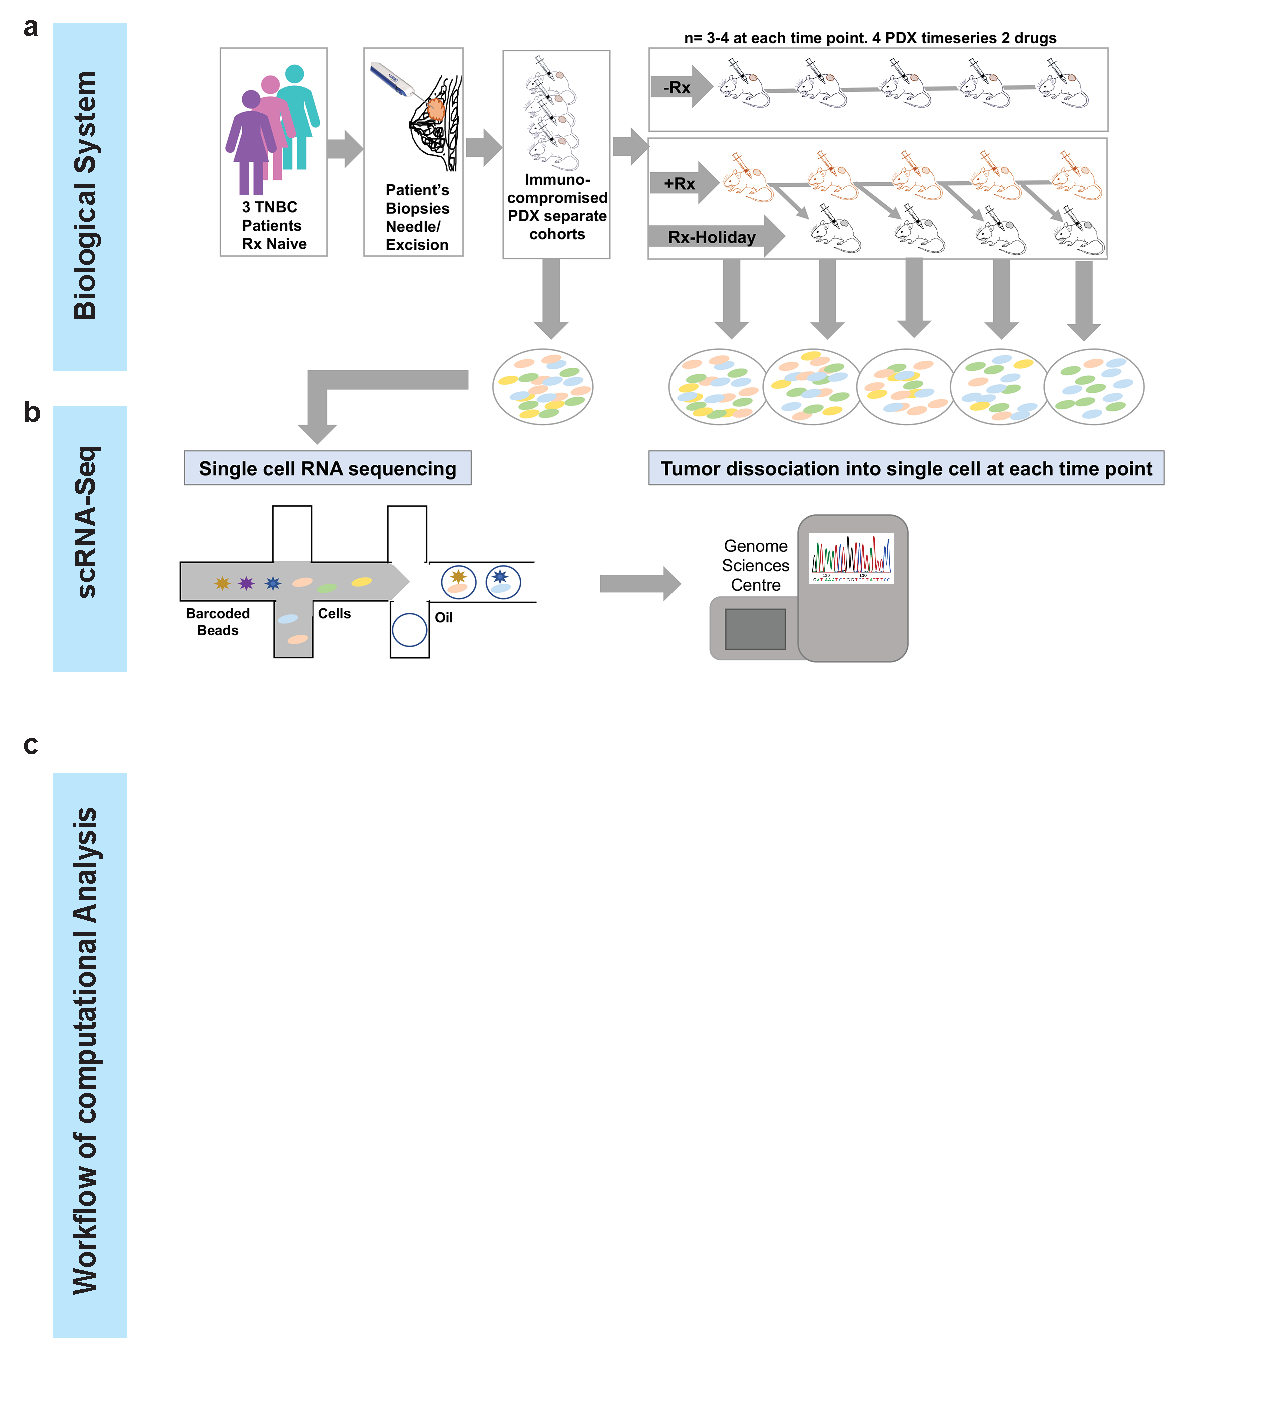
\includegraphics[width=\textwidth]{Figures/fig1schematicsoverview.pdf}
	
\caption[Schematic overview of experimental design and single cell RNA seq data analysis]
	{\small
	 \textbf{Schematic overview of experimental design and single cell RNA seq data analysis} .
	     
	}
	\label{fig:fig1schematicsoverview}
\end{figure}


\section{Results}

\subsection{Clone-specific genotypes underpin clone-specific gene expression programs}
We profiled the impact of clone specific gene expression changes as a higher order representation of phenotypic properties. We tested if the genotypes of high fitness clones exhibited changes in their transcriptional program, with scRNAseq performed on matched aliquots of samples sequenced using DLP+ on the serially passaged triple-negative breast cancer patient-derived xenografts from Chapter 4 as substrates \textbf{\autoref{fig:treatedtimeseriesmanuscript}} and \textbf{\autoref{fig:SA535CX5461} a}.

\subsubsection{Copy number change and scRNAseq expression revealed legitimate correlation across PDX timeseries}
  In our approach, we assume clones are defined through grouped cell subsets which share to a first approximation similar genomic copy number structure (e.g., through phylogenetic reconstruction or dimensionality reduction) \cite{laks2019clonal}. Based on this relationship we applied
  \texttt{clonealign}, a statistical method, \cite{campbell2019clonealign} to reveal clone-specific phenotypic properties across all samples.
  Each point is taken as the proportion of DLP cells in a clone horizontal axis versus the proportion of the scRNAseq cells in the same clone. The  correlation for all clones were then calculated by using Pearson correlation coefficient formula. The heat maps of SA609 TNBC PDX \textbf{(\autoref{fig:UnRxseries} h)} and SA535 TNBC PDX \textbf{(\autoref{fig:SA535analysis} a, e)} exhibit more complex heterogeneity at copy number space along with structural genomic rearrangements as compared to SA1035 TNBC PDX \textbf{(\autoref{fig:SA1035Rxnew} a, e)}. Our results showed DLP+ and \texttt{clonealign} clone abundance measures were positively correlated across all libraries \textbf{(\autoref{fig:fig2_clonealignembeddings.pdf} a, d, g)}. Importantly, SA535 TNBC treated with cisplatin presented the high confidence correlation with Pearson correlation 0.94 (p-value$< 10^{-18}$), followed by its CX-5461 treated series, presenting Pearson correlation of 0.97 (p-value$< 10^{-15}$) \textbf{\autoref{fig:fig2_clonealignembeddings.pdf} g}. However, SA609 PDX timeseries samples present a Pearson correlation coefficient of 0.89 (p-value $< 10^{-16}$) \textbf{(\autoref{fig:fig2_clonealignembeddings.pdf} a)} and SA1035 PDX with Pearson correlation of 0.78 (p-value$< 10^{-18}$) \textbf{(\autoref{fig:fig2_clonealignembeddings.pdf} d)}.
  
  

\begin{figure}
\centering
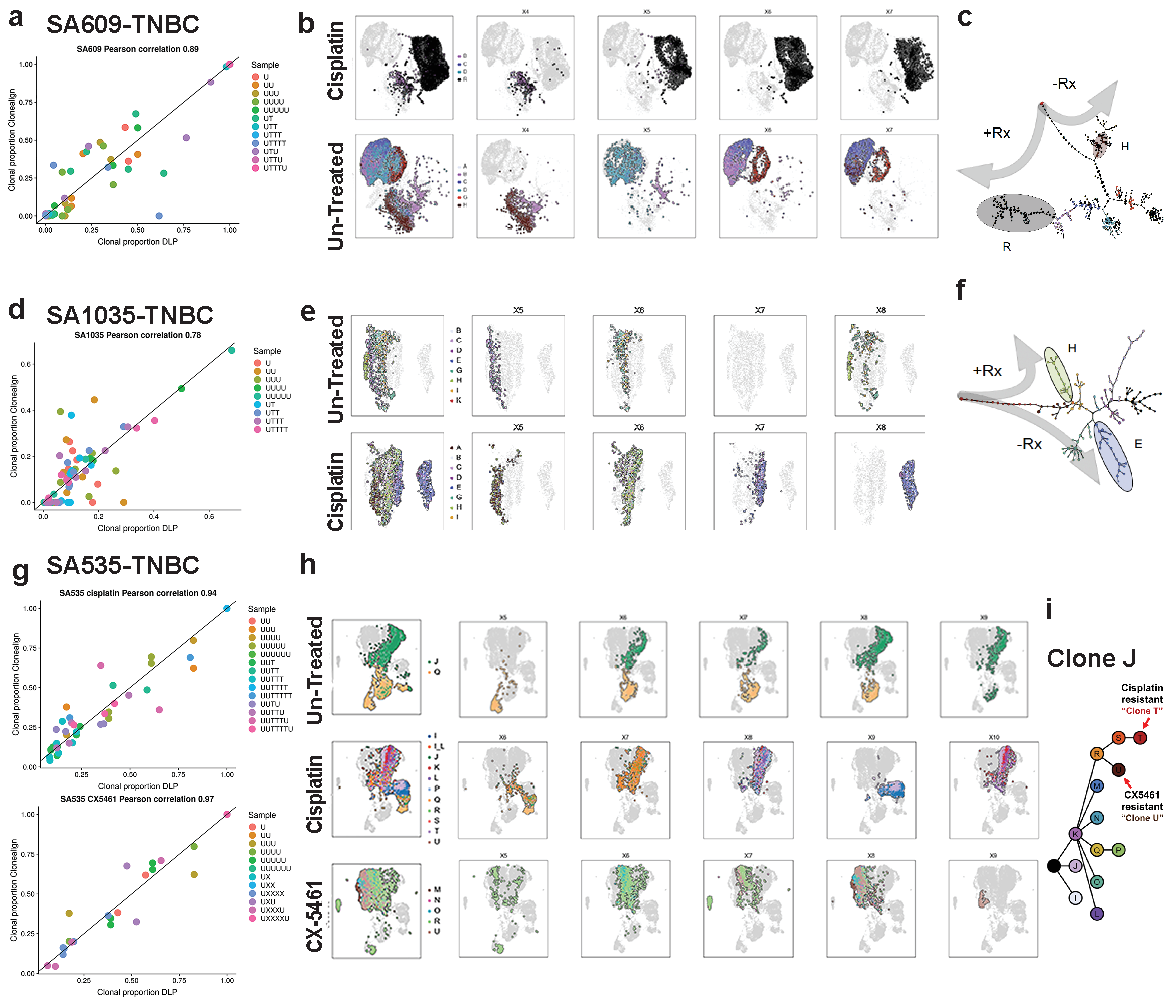
\includegraphics[width=\textwidth]{Figures/fig2_clonealignembeddings.pdf}
	
\caption[Gene expression impacts of clone-specific copy number profiles]
	{\small
	\textbf{Gene expression impacts of clone-specific copy number profiles.}
	   \textbf{(a)} \texttt{clonealign} clonal proportions vs DLP+ clonal proportions of SA609 PDX timeseries samples indicating positive correlation (Pearson correlation from 0.89).
	    \textbf{(b)} Low dimensional \ac{UMAP} embeddings of matching scRNAseq libraries across the SA609 TNBC timeseries. Left top and bottom panels show treated and untreated complete embedding annotated with clonealign assignments and right all panels show the density of cell clusters over the timeseries X4-X7.
	     \textbf{(c)} Phylogeny of SA609 taken from previous chapter to recall emerged clones with or without drug. 
	     \textbf{(d)} Same like \textbf{(a)} but for SA1035 PDX and Pearson correlation is 0.78. \textbf{(e)} Same like \textbf{(b)} but for SA1035 starting from X5-X8. \textbf{(f)} Same like \textbf{c} but for SA1035. \textbf{(g)} Same like \textbf{a} but for SA535 PDX and Pearson correlation is 0.94 for cisplatin treated and 0.97 with CX-5461 treated. \textbf{(h)} Same like \textbf{b} but for SA535 starting from X5-X9, X10.
	}
	\label{fig:fig2_clonealignembeddings.pdf}
\end{figure}



\subsubsection{Single cell RNAseq clusters exhibit relatively monomorphic pattern of global expression over time which tracked with clone assignments}
Next, we visualized the data using UMAP \cite{becht2019dimensionality}, dimensionality reduction method, to aggregate cells into treated and untreated subpopulations while retaining the relationship between subpopulations. scRNAseq embeddings displayed a dynamic pattern of global expression over time with and without treatment, which tracked with clone assignments indicating co-variation of transcriptional properties with clonal abundance \textbf{\autoref{fig:fig2_clonealignembeddings.pdf}}. UMAP visualization of clusters identified clone H clusters in untreated setting and clone R clusters, in the cisplatin treated series of SA609 TNBC PDX, purified over time matching their genomically defined counterparts \textbf{(\autoref{fig:fig2_clonealignembeddings.pdf} b)}. Similarly, clone E in untreated and clone H in treated timeseries of SA1035  \textbf{(\autoref{fig:fig2_clonealignembeddings.pdf} e)}, clustered uniquely at the later time points. \textbf{\autoref{fig:fig2_clonealignembeddings.pdf} c, f} reminding the clones emerging with and without treatment through the phylogeny of DLP+ from chapter 4, in SA609 and SA1035, respectively.  SA535 TNBC PDX all three arms of untreated, treated with cisplatin and CX-5461, exhibited aggregation of similar patterns of clusters that favours emerging of genomic clones in their respective series. Clone J, in untreated control timeseries \textbf{(\autoref{fig:fig2_clonealignembeddings.pdf} h, upper panel)}, clone T, in cisplatin treated \textbf{(\autoref{fig:fig2_clonealignembeddings.pdf} h, middle panel)}, and clone U in CX-5461 treated \textbf{(\autoref{fig:fig2_clonealignembeddings.pdf} h, lower panel)}.

\begin{figure}
\centering
  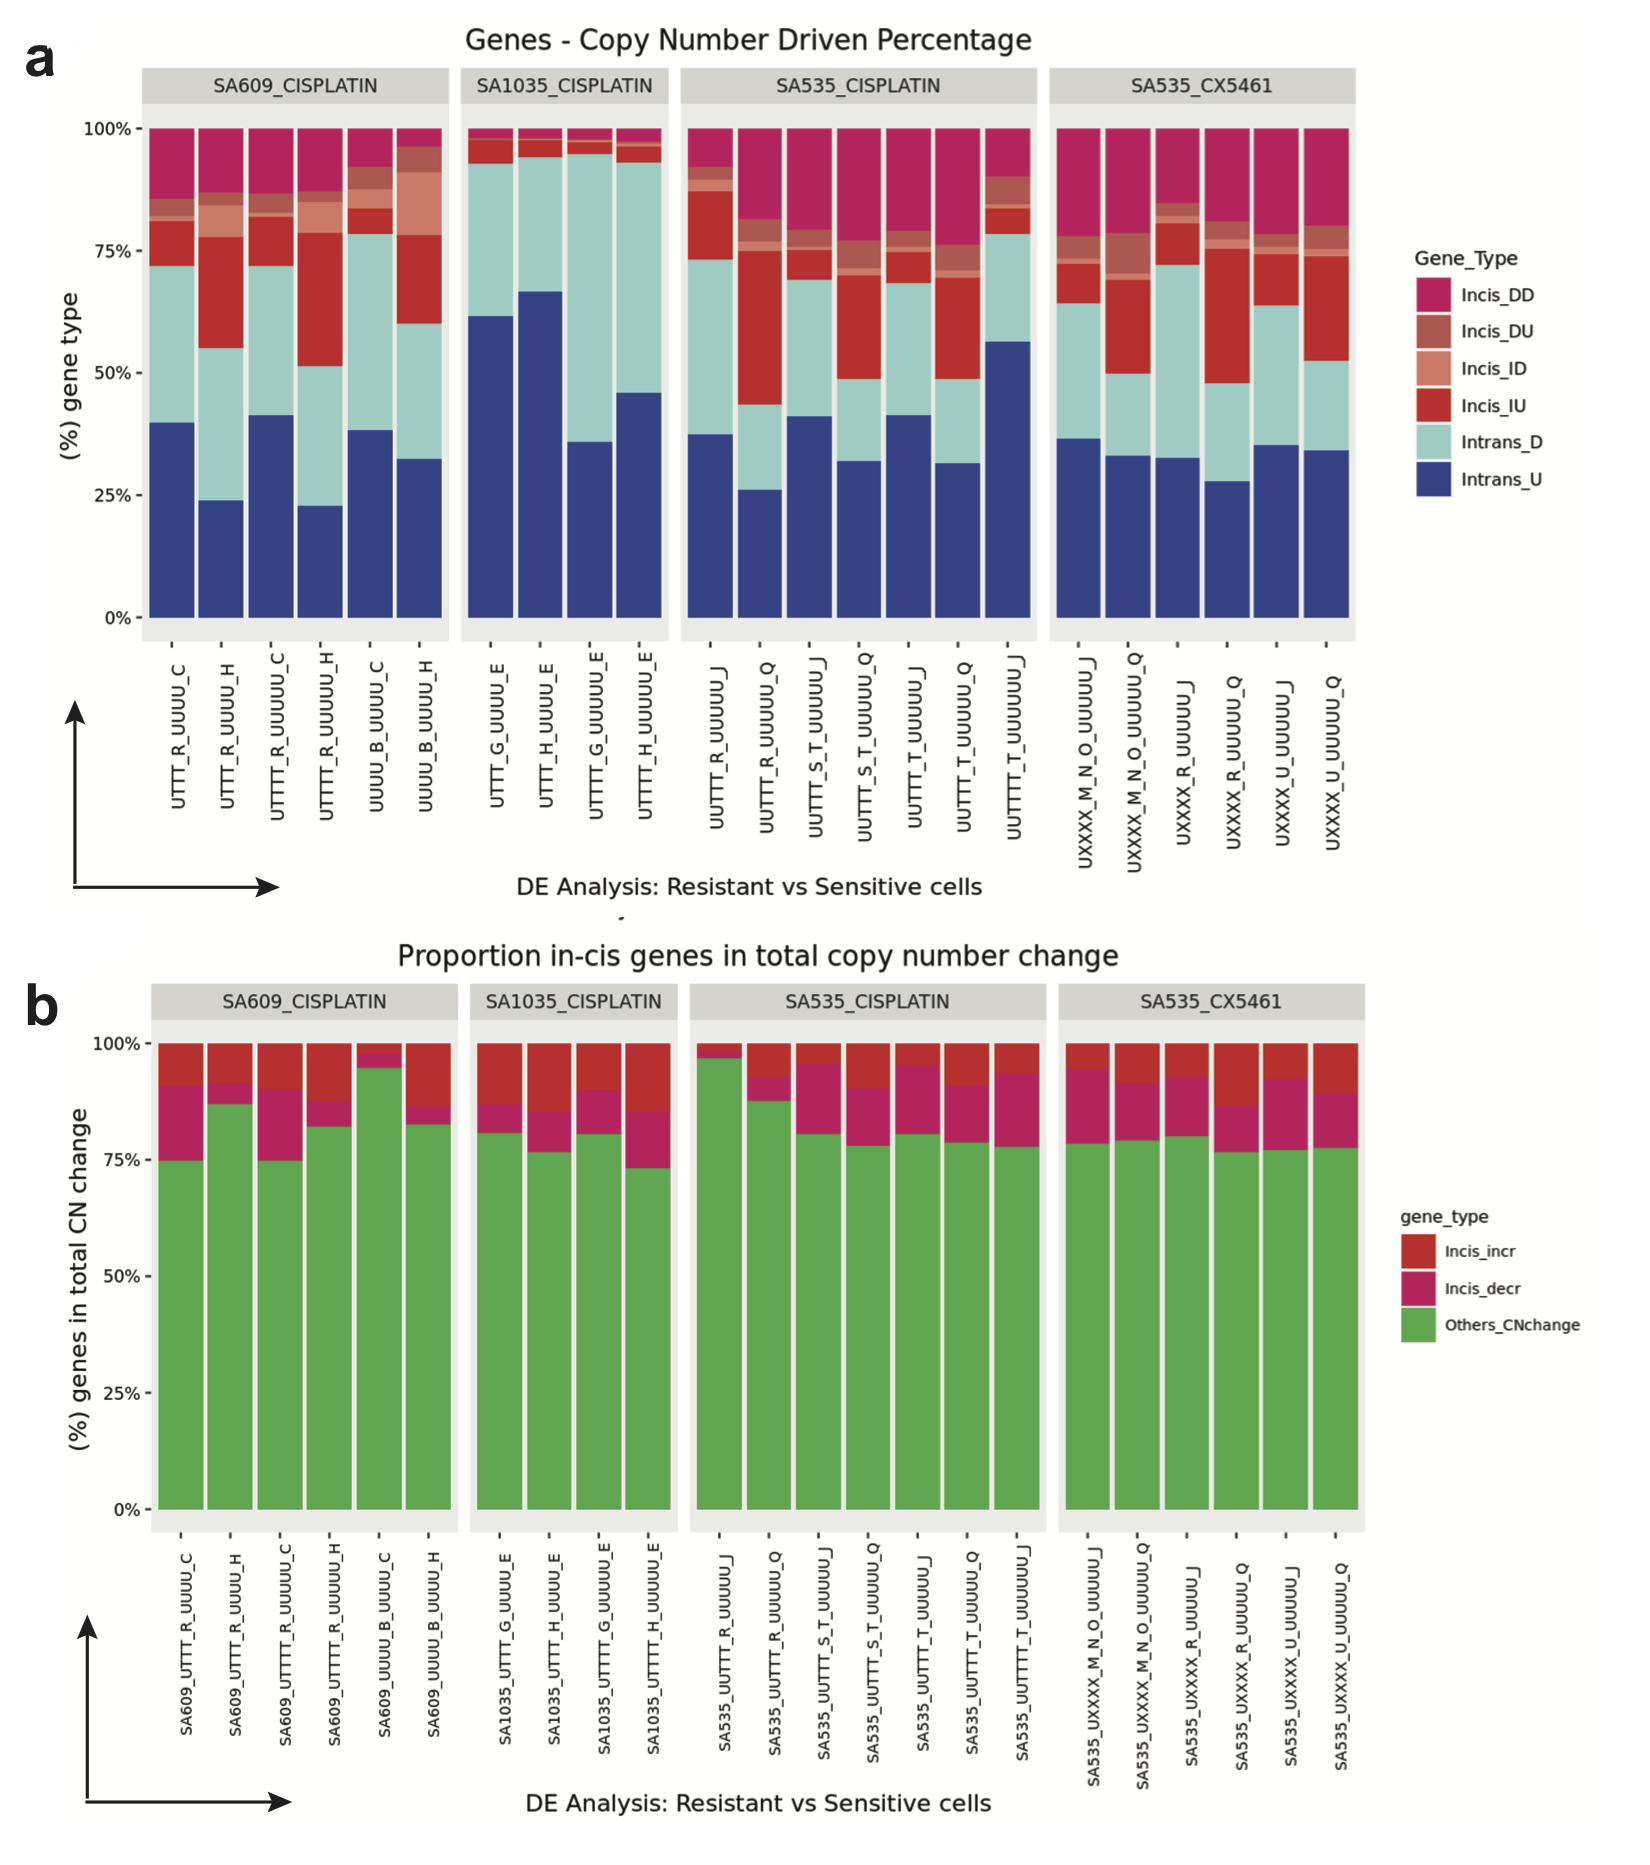
\includegraphics[width=\textwidth]{Figures/fig4Summaryincistrans.pdf}
	
\caption[Summary proportion of \textit{in-cis} and \textit{in-trans} regulated gene expression in scRNAseq data]
	{\small
	\textbf{Summary proportion of \textit{cis} and \textit{trans} regulated gene expression in scRNAseq data.}
	   Horizontal axis shows differential expression between two selected clones from all the three PDX treated and un-treated timeseries. Vertical axis gives percentage presence of genes in-cis or in trans. red bars represent in-cis and blue bars represent in -trans regulated gene expression.
	   \textbf{(a)} This graph gives us percentage of genes by looking into the gene data set from COSMIC cancer gene dataset \cite{vogelstein2013cancer} that corresponds to our clone aware \ac{DE}.
	    \textbf{(b)} same like upper plot but looking into CORE FITNESS data set \cite{behan2019prioritization}.
	     
	}
	\label{fig:fig3Summaryincistrans}
\end{figure}



\subsection{Quantitative single cell gene expression analysis unravels the rates of \textit{ in cis} and \textit{in trans} components}
Next, we investigated the proportions of \textit{in cis} and \textit{in trans} regulated genes in our procured single cell RNA expression data but within selected \ac{DE} of clones across all timeseries. From HMMcopy output of segment copy number position (chromosome start and end), we get gene coordinate by map our segment positions with reference database of known genes for human  \cite{carlson2015txdb}. First, we identify overlapping positions between chromosome segment and known genes, then we assigned that segment to an ensemble gene ID \cite{rainer2019ensembldb}.

Total of 22,326 segment positions, from each DE analysis, were mapped. In each pair wise comparison of clones, we captured all segment copy number position where there is a change in copy number values. So \textit{in-cis} gene is DE gene in scRNAseq analysis and coupled with change in copy number at the same position of genome HMM copy number segment positions.

\subsubsection{Single cell RNAseq global proportion of resistant vs sensitive clones presented high \textit{in trans}-regulated gene expression variations than \textit{in cis}-regulated genes} 

To calculate the percentage of genes presenting \textit{in cis} or \textit{in trans} regulatory effects, the differential expression single cell RNAseq data was decomposed into \textit{cis}, where the gene expression that is following the change in copy number and \textit{trans}, where it is independent. Then, we classified the common genes into  \textit{cis}  and \textit{trans} genes and calculated their number and percentages in each PDX timeseries. 

The average change in copy number between the genomes of two clones in our data set was found to be around 41\%. Out of this approximately 28\% of the transcriptome is coupled with change in copy number state between clones. It involves either increase in expression with copy number gain or decrease in expression with copy number loss, shown in pink and red for \textit{in cis} and rest of  around 72\% of the others in green as shown in  \textbf{(\autoref{fig:fig3Summaryincistrans} a)}.

% Please add the following required packages to your document preamble:
% \usepackage{graphicx}
% \usepackage{lscape}
\begin{landscape}
\begin{table} 
\centering
 \caption{Summary of \textit{in cis} and \textit{in trans} percentages(\%)}
\resizebox{\textwidth}{!}{%
\begin{tabular}{|l|p{5em}|p{5em}|p{5em}|p{5em}|p{5em}|p{5em}|}
  \hline
\ac{DE}-scRNAseq &
  In\_cis\_Decrease\_DownRegulated &
  In\_cis\_Decrease\_UpRegulated &
  In\_cis\_Increase\_DownRegulated &
  In\_cis\_Increase\_UpRegulated &
  In\_trans\_DownRegulated &
  In\_trans\_UpRegulated \\
    \hline
SA609\_UUUU\_B\_UUUU\_C         & 7.9  & 4.4 & 4   & 5.2  & 40.1 & 38.4 \\
SA609\_UUUU\_B\_UUUU\_H         & 3.5  & 5.1 & 13  & 17.5 & 27.7 & 33.2 \\
SA609\_UTTT\_R\_UUUU\_C         & 14.4 & 3.3 & 1.1 & 9.3  & 32.1 & 39.8 \\
SA609\_UTTT\_R\_UUUU\_H         & 13   & 2.5 & 6.5 & 22.5 & 31.3 & 24.2 \\
SA609\_UTTTT\_R\_UUUUU\_C       & 13.2 & 3.8 & 0.9 & 10.1 & 30.5 & 41.5 \\
SA609\_UTTTT\_R\_UUUUU\_H       & 12.8 & 2.2 & 6.1 & 27.1 & 28.7 & 23   \\
SA1035\_UTTTT\_G\_UUUUU\_E      & 1.8  & 0.2 & 0.4 & 2.3  & 59.2 & 36.2 \\
SA1035\_UTTTT\_H\_UUUUU\_E      & 2.6  & 0.5 & 0.5 & 3.3  & 47.2 & 45.8 \\
SA1035\_UTTT\_G\_UUUU\_E        & 1.6  & 0.1 & 0.1 & 4.8  & 31.5 & 61.9 \\
SA1035\_UTTT\_H\_UUUU\_E        & 1.9  & 0.3 & 0.3 & 3.4  & 27.4 & 66.7 \\
SA535\_UUTTTT\_T\_UUUUUU\_J     & 9.7  & 5.6 & 0.3 & 3.2  & 22.8 & 58.3 \\
SA535\_UUTTT\_T\_UUUUU\_J       & 20.9 & 3.4 & 0.2 & 4.5  & 27.6 & 43.3 \\
SA535\_UUTTT\_S\_T\_UUUUU       & 20.7 & 3.4 & 0.2 & 4.4  & 28.3 & 43   \\
SA535\_UUTTT\_R\_UUUUU\_J       & 7.9  & 2.5 & 1.5 & 12.3 & 36.8 & 39.1 \\
SA535\_UUTTT\_T\_UUUUU\_Q       & 22.5 & 4.9 & 1.5 & 20.7 & 18.4 & 32   \\
SA535\_UUTTT\_S\_T\_UUUUU\_2    & 21.7 & 5.2 & 1.4 & 21.2 & 18.1 & 32.4 \\
SA535\_UUTTT\_R\_UUUUU\_Q       & 16   & 4.4 & 1.8 & 31.5 & 19.9 & 26.4 \\
SA535\_UXXXX\_U\_UUUUU\_J       & 21.5 & 2.8 & 0.6 & 8.8  & 29.2 & 37.1 \\
SA535\_UXXXX\_U\_UUUUU\_Q       & 18.1 & 4.4 & 1.6 & 21.4 & 20.1 & 34.5 \\
SA535\_UXXXX\_R\_UUUUU\_J       & 15.3 & 2.4 & 0.6 & 7    & 40.4 & 34.3 \\
SA535\_UXXXX\_R\_UUUUU\_Q       & 17.1 & 3.4 & 1.9 & 27.5 & 21.8 & 28.2 \\
SA535\_UXXXX\_M\_N\_O\_UUUUU\_J & 22.1 & 4.3 & 0.4 & 6    & 28.5 & 38.7 \\
SA535\_UXXXX\_M\_N\_O\_UUUUU\_Q & 19.7 & 7.7 & 1.3 & 19.3 & 18.6 & 33.5 \\
  \hline
 \end{tabular}%
}
\end{table}
\end{landscape}

Next, we 







\begin{figure}
\centering
  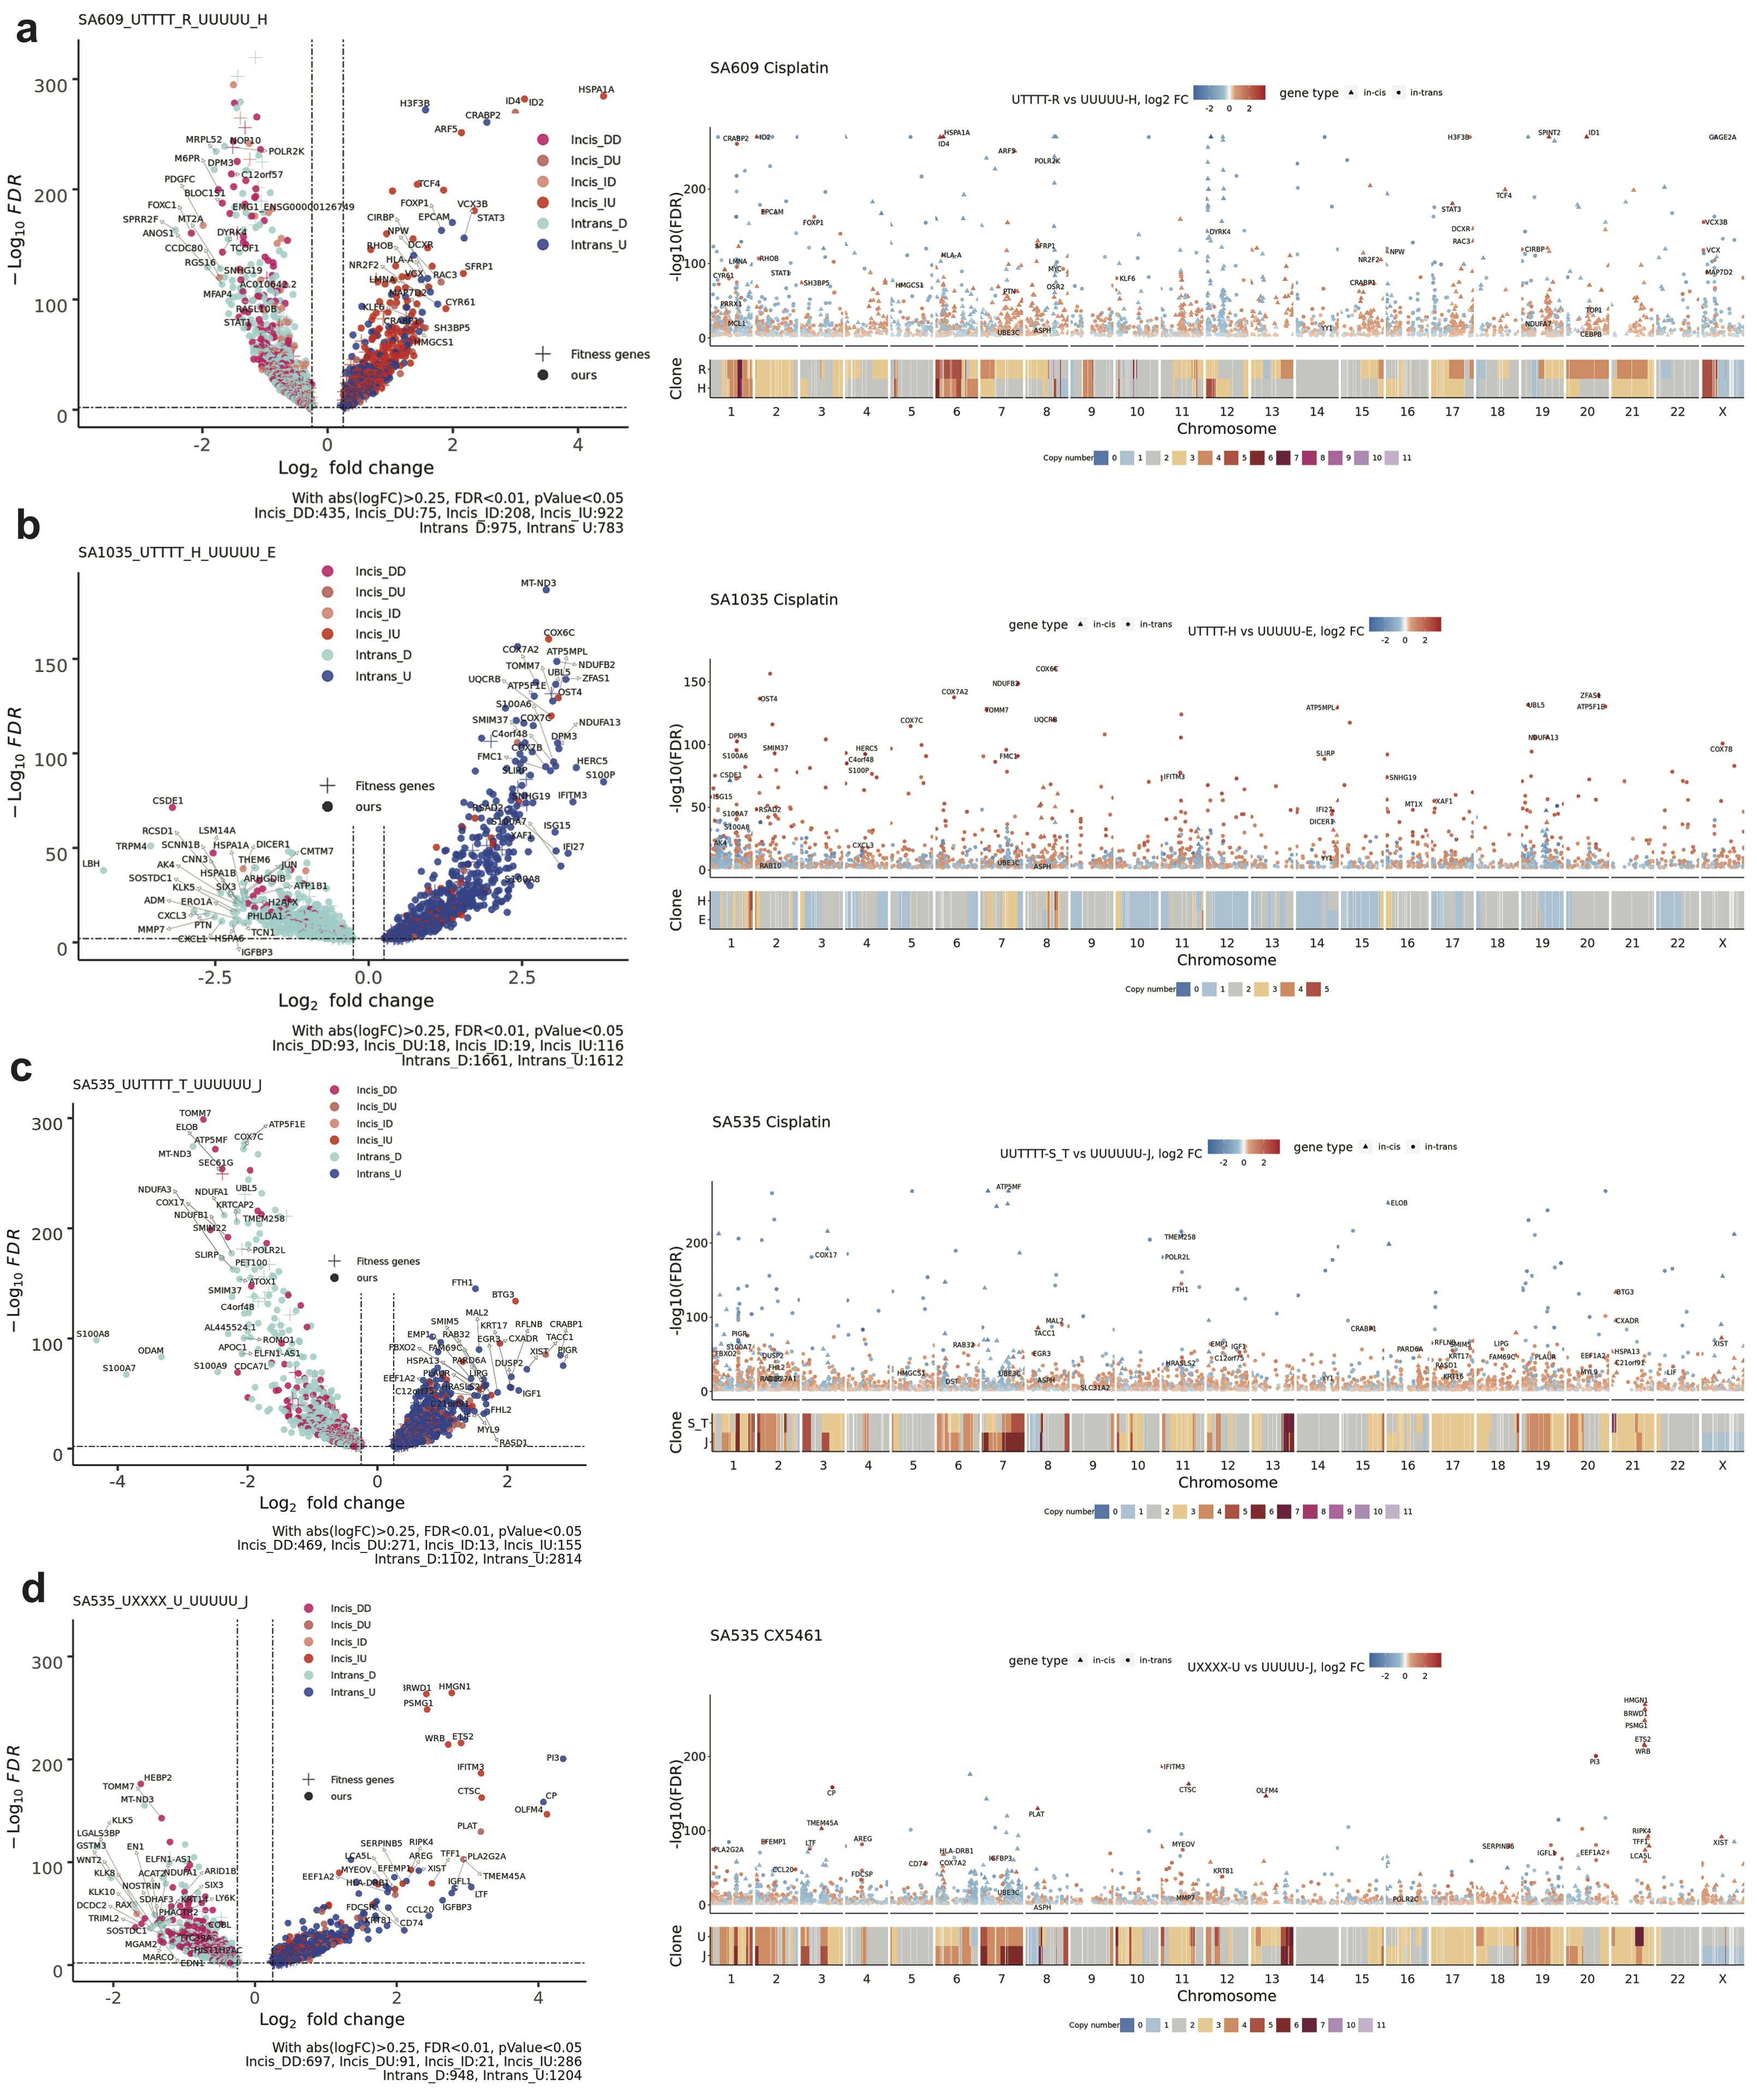
\includegraphics[width=\textwidth]{Figures/Volcanotrackplots2.pdf}
\caption[DE of resistant and sensitive clonealign defined clones]
	{\small
	\textbf{Differential expression of resistant and sensitive clones.}
	\textbf{(a)} Volcano plot from SA609 -log10(FDR) plotted against log2 fold change of pairwise differential gene expression between resistant and sensitive clones. (The threshold for significant genes are FDR p$<$00.01, P Value p$<$00.05, logFC p$>$0 0.25). Manhattan plot (genome-wide view) of differential gene expression between pairs of clones, R vs H corresponding to change in gene expression (Right).
	    \textbf{(b)} Same like \textbf{a} but in SA1035 and comparing between pairs of clones, H vs E. 
	     \textbf{(c)} Same like \textbf{a} but in SA535 (cisplatin) and comparing between pairs of clones, S\_T vs J.
	      \textbf{(d)} Same like \textbf{a} but in SA535 (CX-5461) and comparing between pairs of clones, U vs J.
	 
	   }
	\label{fig:fig4_Volcanotrackplots2.pdf}
 \end{figure}

\begin{figure}
\centering
  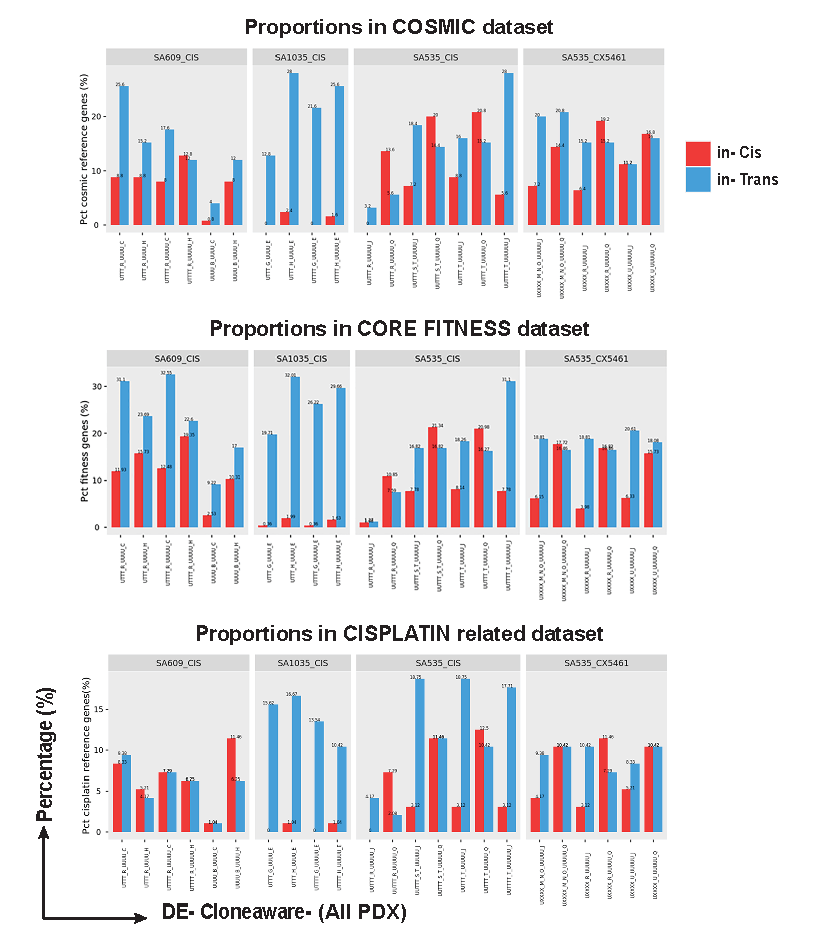
\includegraphics[width=\textwidth]{Figures/fig3_In_cispercentage.pdf}
	
\caption[Proportion of \textit{in-cis} and \textit{in-trans} regulated gene expression in scRNAseq data]
	{\small
	\textbf{Proportion of \textit{cis} and \textit{trans} regulated gene expression in scRNAseq data.}
	   Horizontal axis shows differential expression between two selected clones from all the three PDX treated and un-treated timeseries. Vertical axis gives percentage presence of genes in-cis or in trans. red bars represent in-cis and blue bars represent in -trans regulated gene expression.
	   \textbf{(Upper)} This graph gives us percentage of genes by looking into the gene data set from COSMIC cancer gene dataset \cite{vogelstein2013cancer} that corresponds to our clone aware \ac{DE}.
	    \textbf{(Middle)} same like upper plot but looking into CORE FITNESS data set \cite{behan2019prioritization}.
	     \textbf{(Lower)} Same like above but looking into cisplatin related gene list curated from literature.
	    
	}
	\label{fig:fig3_In_cispercentage}
\end{figure}

\subsubsection{Differential expression analysis of resistant and sensitive clones deciphers cancer related genes}
 Next, we sought to explore individual genes that are differentially expressed  between the resistant and sensitive clones of all four treatment regimes in all PDX in the above data. 
 Pairwise comparisons of clone-specific differential gene expression in SA609, resistant (Clone R) and sensitive (Clone H) clone (FDR$<$0.01, p$<$0.05) identified 922 genes having clone specific copy number increase in expression, whereas, 435 genes were downregulated with decrease in copy number. However, 850 genes were downregulated and 738 were upregulated and 975 were downregulated \textit{in trans} \textbf{(\autoref{fig:fig4_Volcanotrackplots2.pdf} a)}.  Amidst the upregulated \textit{in cis}, some known cancer promoting genes were detected, for example, HSPA1 \cite{zoppino2018comprehensive}, TCF4 \cite{ravindranath2011wnt}, NDUF \cite{li2015down}, PTN \cite{huang2018chemotherapy}, ID4 \cite{donzelli2018expression}, RAC3 \cite{donnelly2017rac3}. Additionally, \textit{in cis} downregulated genes includes genes that have role in tumor suppression, for example, OSR2, is known tumor suppressor in gastric and lung cancer \cite{otani2014odd,wang2018odd}. Other genes include, DYRK4 is found to be downregulated in our data and is a key regulator
of p53, and phosphorylates it at Ser46 to induce apoptosis in response to
DNA damage \cite{yoshida2019multiple}, POLR2K is a candidate biomarker for predicting breast cancer immunotherapy \cite{lopez2020prediction}. Another gene, PRRX1 predicts poor prognosis in hepatocellular carcinoma via the p53-dependent signaling pathway predicts poor prognosis in hepatocellular carcinoma \cite{fan2017downregulation}. Moreover,
KLF6 is found to be among the upregulated genes, which is associated with poor prognosis in prostate, lung, ovarian cancer and breast cancer \cite{hatami2013klf6,difeo2009role}, RHOB \cite{ju2018rhob},
STAT3 \cite{li2019clinicopathological,kamran2013role} and 
ARF5 \cite{li2017roles,casalou2020role} promotes cancer cell survival, migration and invasion. HMGCS \cite{chen2017hmgcs2} mRNA expression is associated with poor clinical prognosis and outcomes in
patients with colorectal cancer (CRC) and oral squamous cell carcinoma (OSCC). NR2F2 is also found upregulated in resistant clone and is known for a worse prognosis and lymph node metastasis in human breast cancer \cite{erdHos2020nr2f2,xia2020nr2f2},
M6PR is frequently down-regulated or inactivated by mutations in a broad range of malignant human cancers \cite{dalle2018mannose} found to be down regulated in the resistant clone.

CRABP2 can suppress invasion and metastasis of ER+ breast cancer 


 
In SA1035 resistant versus sensitive DE plots shows  


 COX6C \cite{yang2018overexpression,chang2017estrogen}
 UQCRB \cite{kim2017mitochondrial,park2017mitochondrial} novel prognostics markers in colorectal and hepatocellular carcinoma.
 ATP5MPL, prognostic factor in ovarian cancer
 CXCL3 \cite{gui2016overexpression, karin2020cxcr3}
CSDE1 \cite{martinez2019unr}
AK4 \cite{jan2019co}


SA535-cisplatin

TACC1 \cite{shakya2018high} hepatocellular carcinoma.
DST  \cite{salerno2016human}
HMGCS1 \cite{walsh2020mevalonate}
TAGLN \cite{wu2014transgelin, elsafadi2020transgelin}
KRT16 \cite{huang2019novel}
IFITM3 \cite{liu2019ifitm3}
S100A7 \cite{zhang2019clinical, mayama2018olfm}
CYP27A1  \cite{liang2019cyp27a1, wu201327}
SLC31A2 \cite{bai2017structural}, membrane transporters downregulated

SA535-CX-5461
MMP7 \cite{mcgowan2008matrix} correlated with cancer invasion, metastasis, and poor prognosis,
TMEM45A \cite{schmit2019characterization} chemoresistance in breast cancer
ETS2 \cite{ge2008role} functions as an oncogene and plays a key role in the progression of hypopharyngeal cancer and associated with poor prognosis \cite{fu2017high}.
COX7A2 \cite{deng2018overexpression} is downregulated in resistant clone which is negatively correlated with prognosis
POLR2C \cite {moriwaki2017polr2c} mutation is known to progress ovarian cancers and its found downregulated in resistant clone.
OLFM4 \cite{ashizawa2019olfm4} is reported to be highly expressed in cancers, including gastric cancer, colon cancer, and pancreatic cancer and to promote tumor progression by inducing cell‐cycle progression and enhancing tumor invasion and metastasis.


\subsubsection{Measuring \textit{in cis} and \textit{in trans} proportions in various gene lists}
First we pulled the reference genes  intersecting with our \ac{DE} data from the three lists (COSMIC \cite{vogelstein2013cancer}, core cancer fitness \cite{behan2019prioritization} and cisplatin related genes curated from last 10 years literature \textbf{\autoref{tab:Cisplatinrelatedgenes}}.

 In  SA609 TNBC PDX, the mean number of \textit{in cis} genes was 1173.8 (segment positions, $\sigma$ = 494 \textit{in cis} genes, max= 1640, min=215), SA1035 presented with the lowest \textit{in cis} with
 mean value of 187.8 (segment positions, $\sigma$ = 51 \textit{in cis} genes, max=246, min=144). SA535 in cisplatin timeseries showed mean number of 1056.9 \textit{in cis} genes (segment positions, $\sigma$ = 624 , max=1900, min=116), whereas, SA535 in CX-5461 exhibit highest number of mean \textit{in cis} value of 1400.7 (segment positions, $\sigma$ = 481 \textit{in cis} genes, max=1884, min=739).
 
 Overall, our results remained consistent with the fact that the proportion of \textit{in trans} regulation of gene expression is higher than the \textit{in cis} in all the time series PDXs and from all the reference lists.   
 
 Interestingly, we noticed that SA535 TNBC in both treatment regimes, inferred highest rate of \textit{in cis} genes with 28\% maximum, whereas, SA1035 TNBC possessing the lowest rate of 2.4\% maximum. SA609 TNBC showed 12.8\% of its highest \textit{in cis} gene rate \textbf{\autoref{fig:fig3_In_cispercentage}}.





\subsection{Integrated transcriptome and pathway analyses revealed potential crucial genes and key pathways in breast cancer}

\subsubsection{Transcriptomic profiling capture key pathways up-down regulation in resistant and sensitive clones}

\subsubsection{Gene co-expression network analysis apprise biological processes relationship}
  

\subsubsection{Gene specific expression trajectories exemplified systematic response to sustained treatment}



\begin{figure}
\centering
  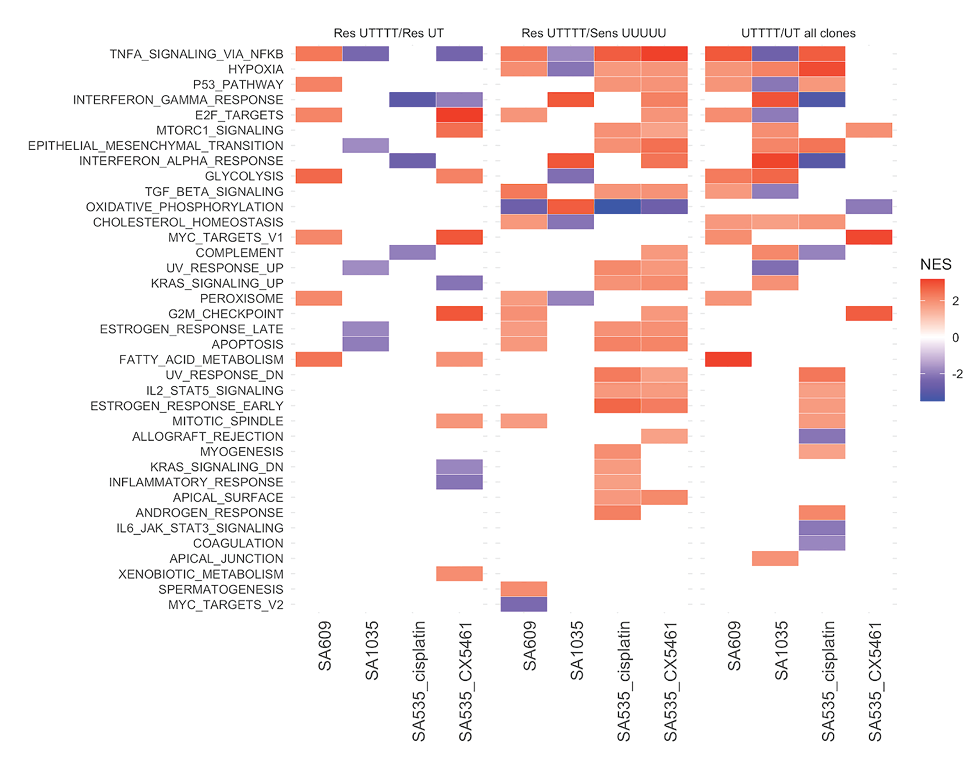
\includegraphics[width=\textwidth]{Figures/fig5pathwaysnetwork.pdf}
\caption[Pathways enrichment analysis of PDX timeseries]
	{\small
	\textbf{Pathways enrichment analysis of PDX timeseries.}
	 Vertical axis on the left enlisting the pathways involved under various conditions in timeseries PDXs. Left panel comparing resistant clone versus clone exposed to only one cycle of drug. Middle panel comparing resistant versus sensitive clone in all PDXs. Right panel comparing last treated timepoint as a whole with first treated timepoint. Horizontal axis is showing the names of PDXs.
	}
	\label{fig:fig5pathwaysnetwork}
\end{figure}

\begin{figure}
\centering
  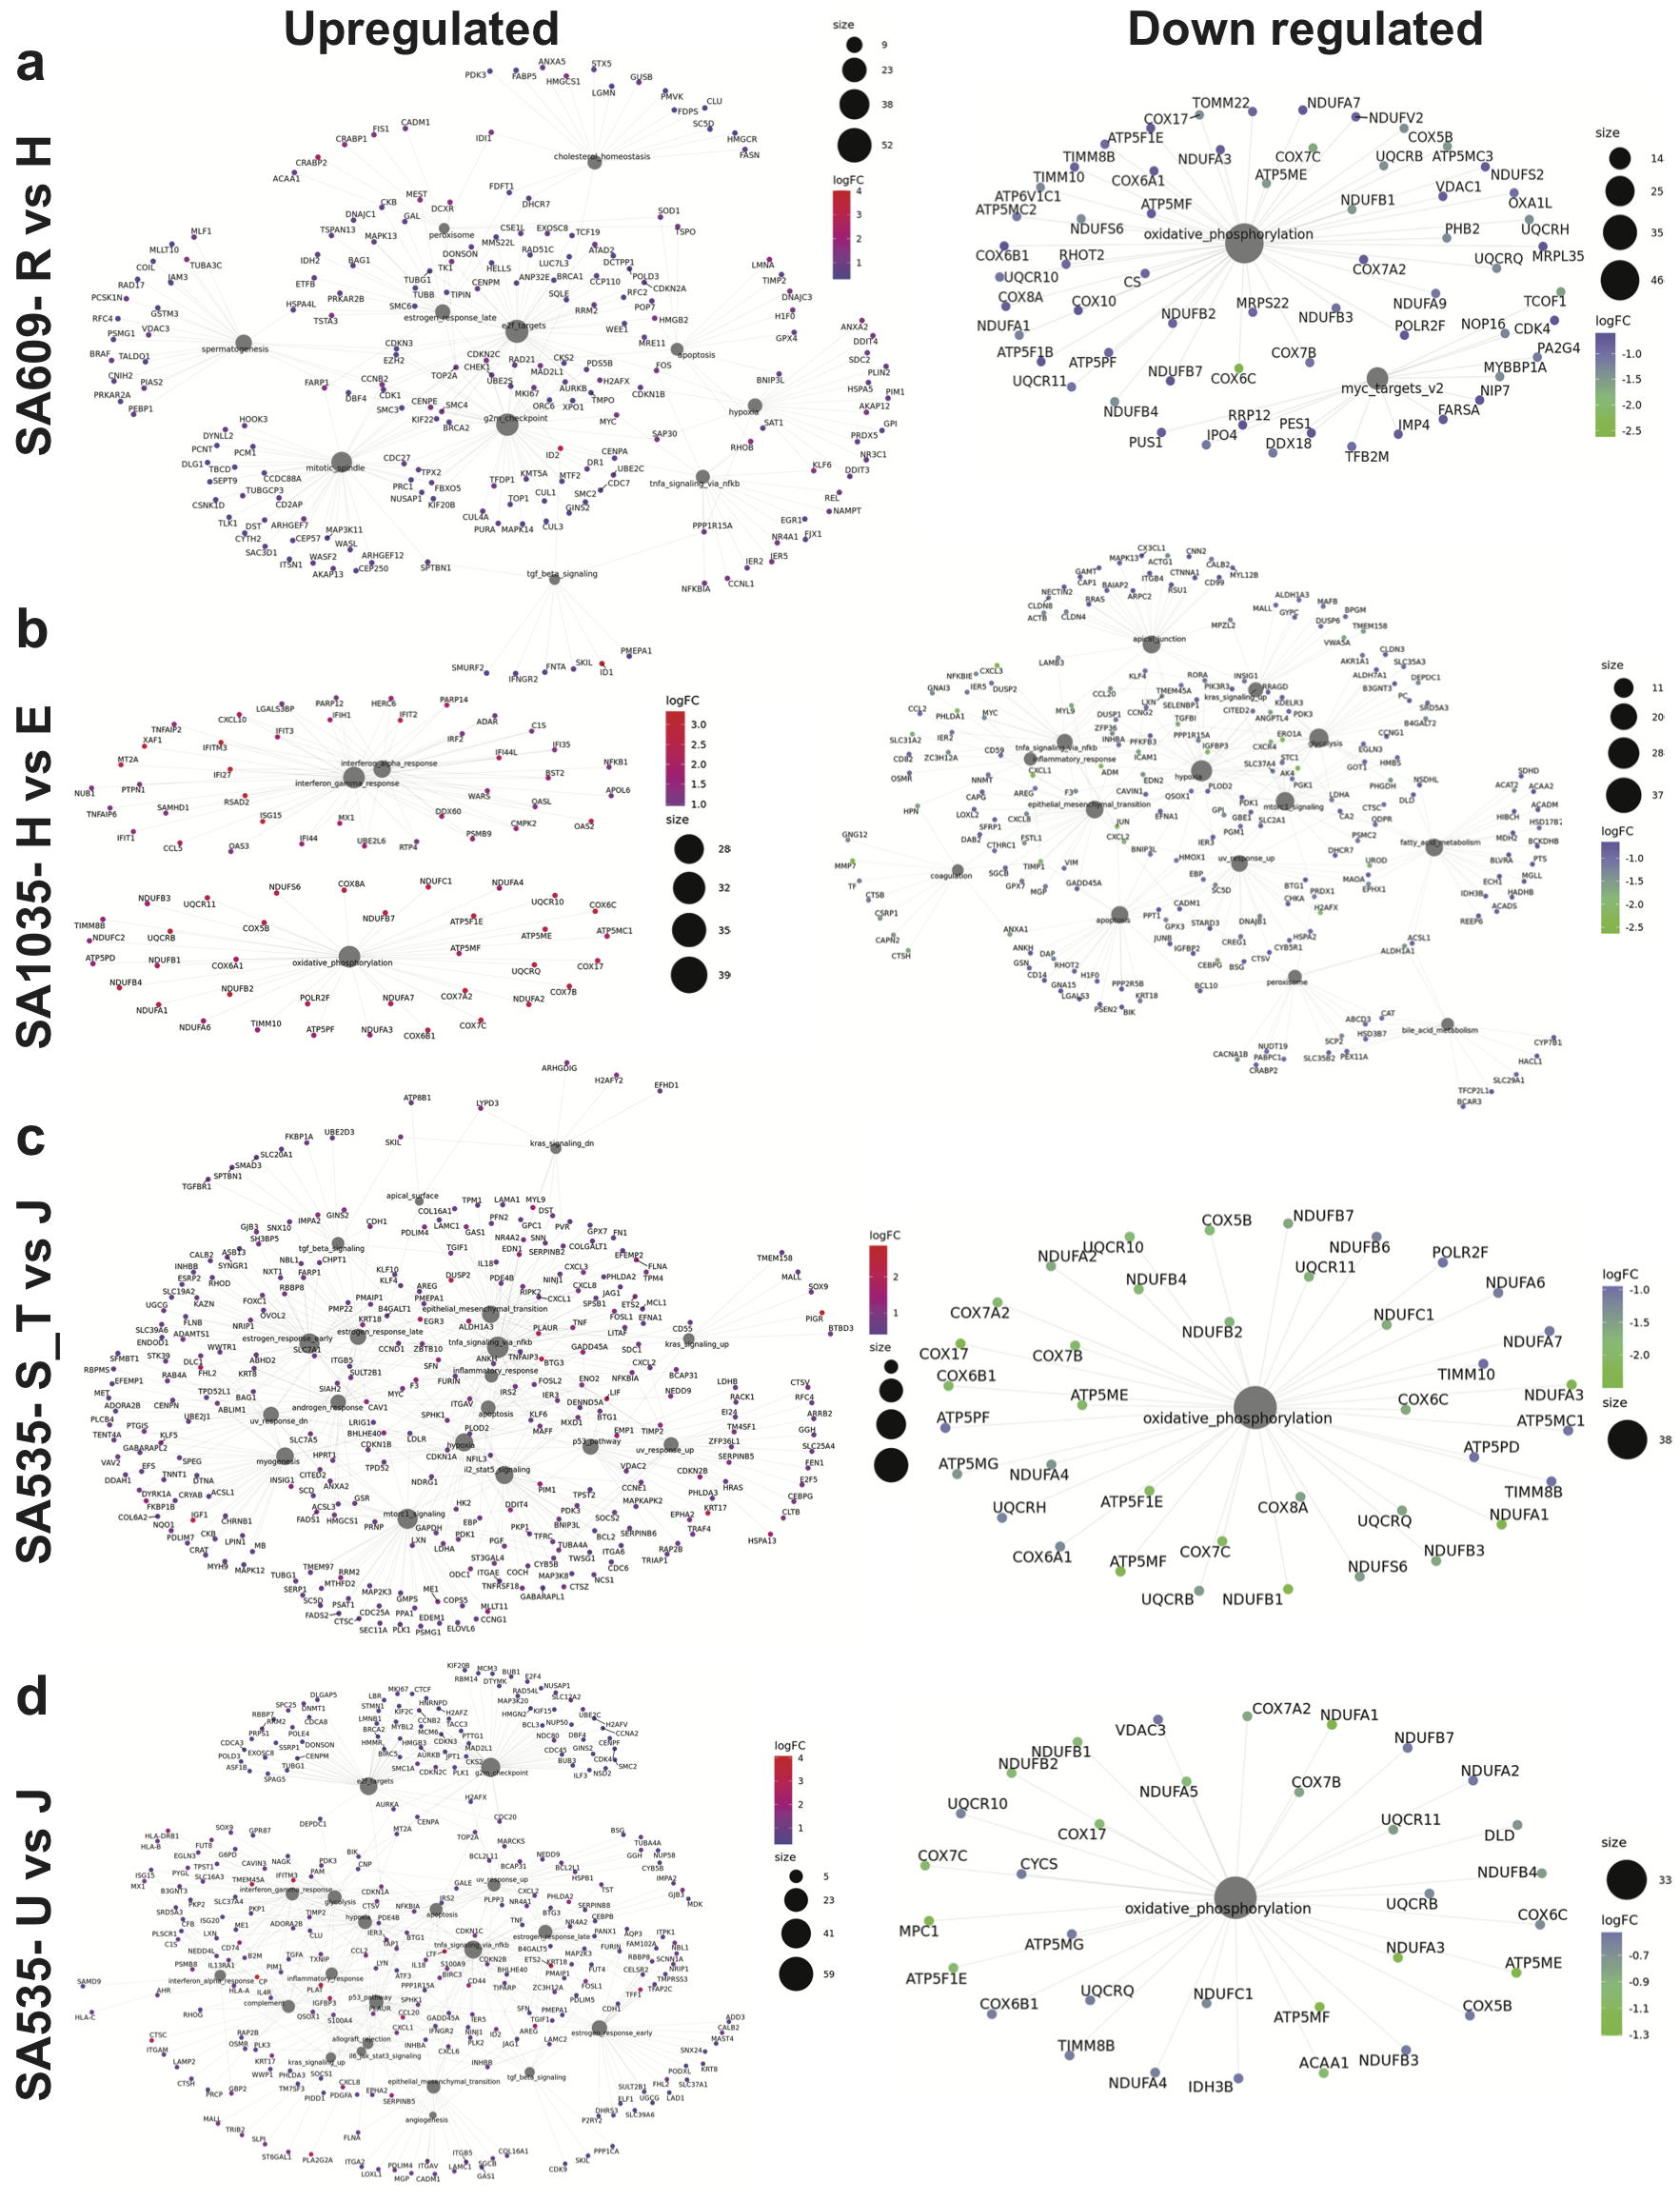
\includegraphics[width=\textwidth]{Figures/genenetworkanalysis.pdf}
\caption[DE of resistant and sensitive clonealign defined clones]
	{\small
	\textbf{Pathway enrichment network comparing resistant and sensitive clones across timeseries PDX.}
	\textbf{(a)} Normalized enrichment score of Pathways between resistant and sensitive clone of all treated timeseries PDXs.
	    \textbf{(b)} Pathway enrichment network comparison of clone }
		\label{fig:genenetworkanalysis}
\end{figure}




 \begin{figure}
\centering
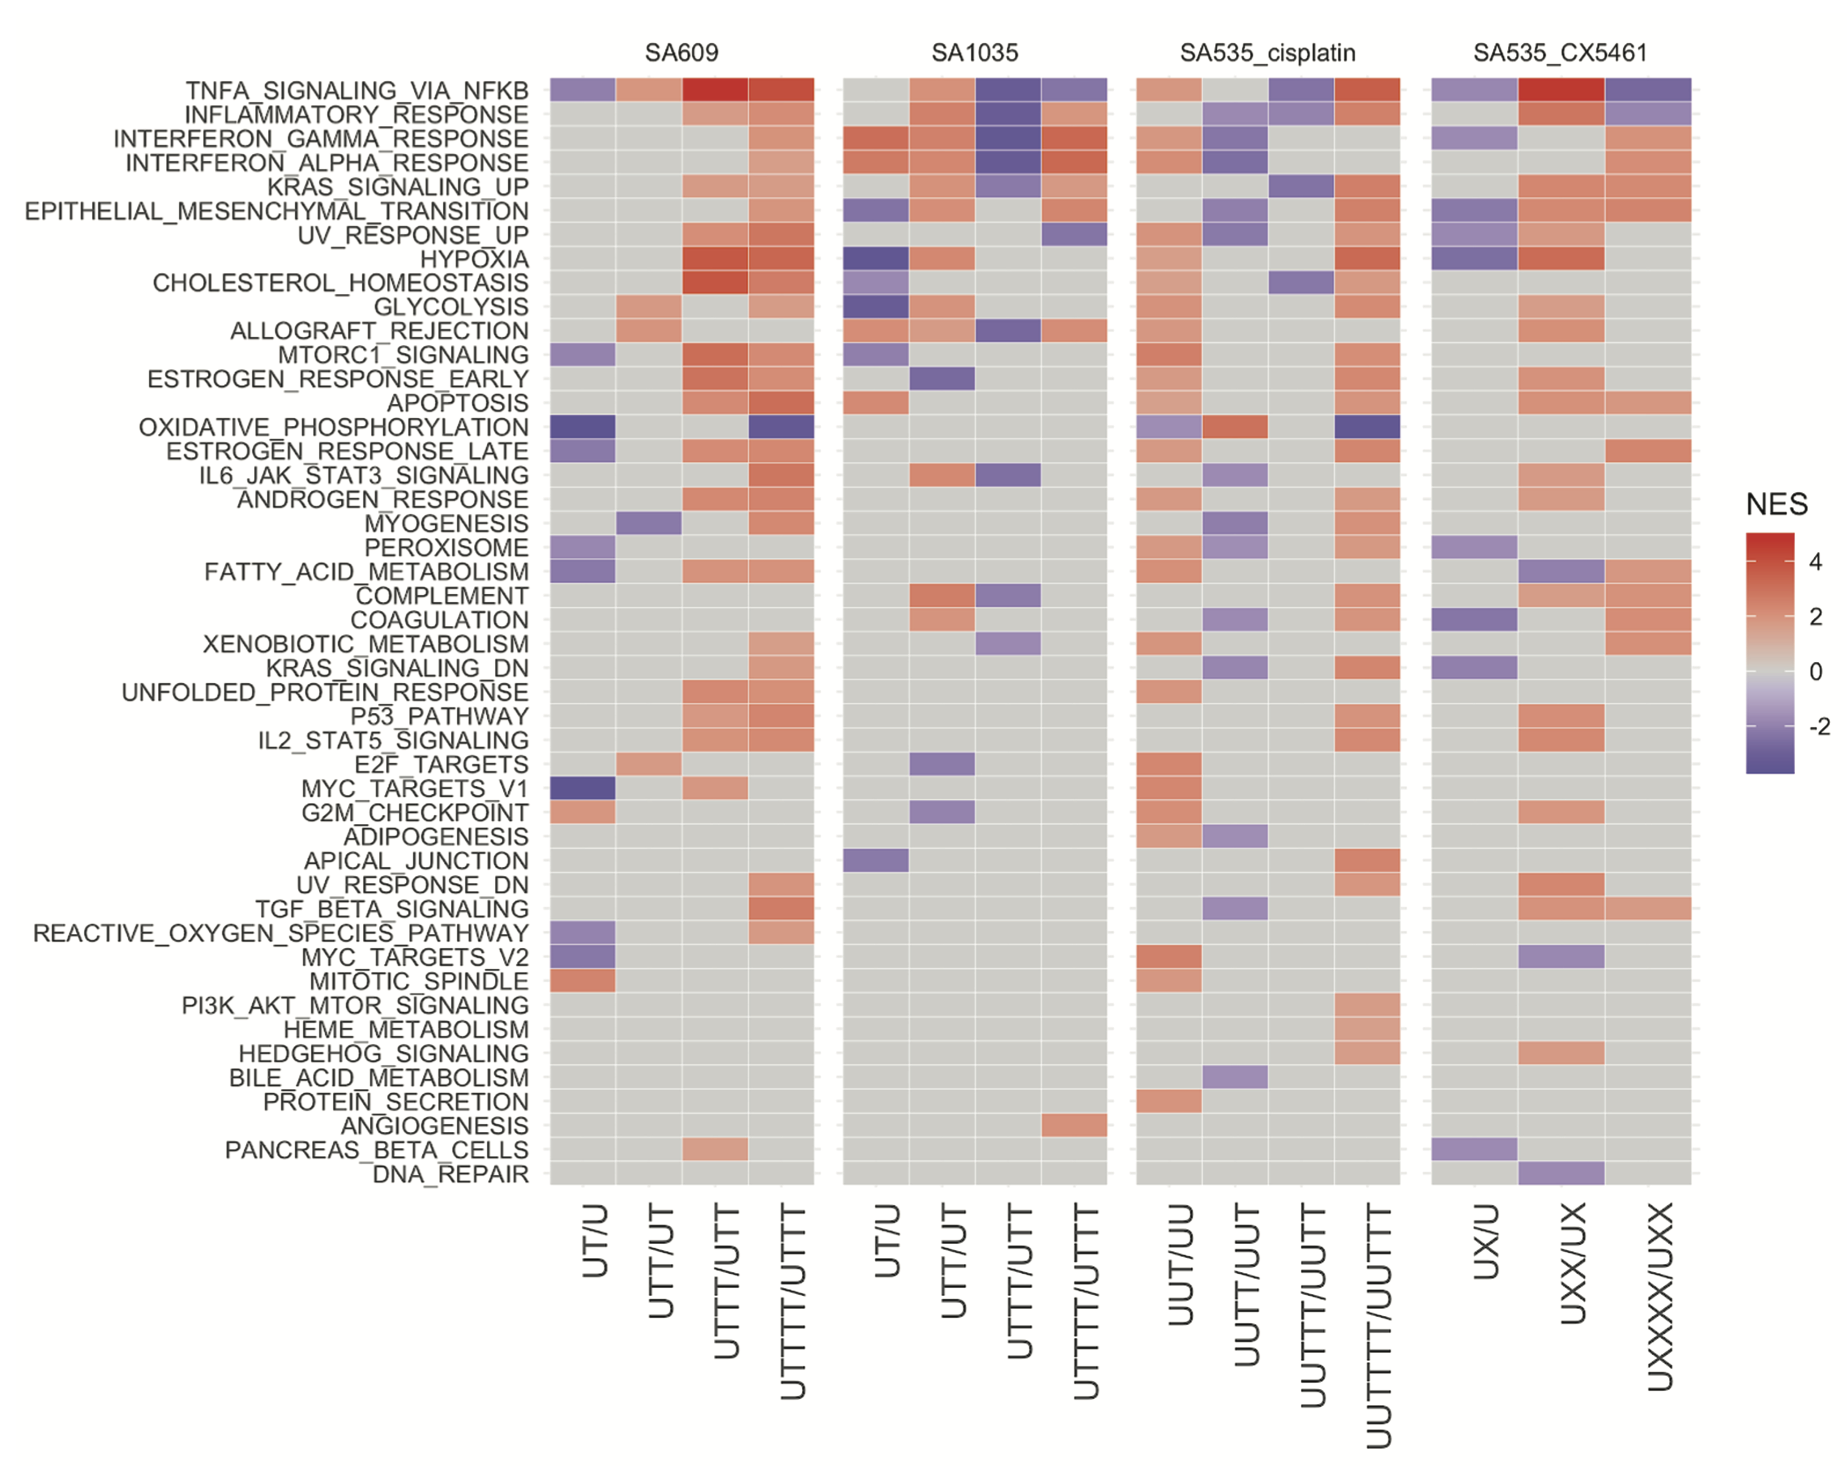
\includegraphics[width=\textwidth]{Figures/pathwaysevolution.pdf}
\caption[Summary of number of genes \textit{in-cis} and \textit{in-trans}]
	{\small
	\textbf{Pathways comparison over time in all PDX series}
	
}
    \label{fig:pathwaysevolution}
    \end{figure}






\begin{figure}
\centering
 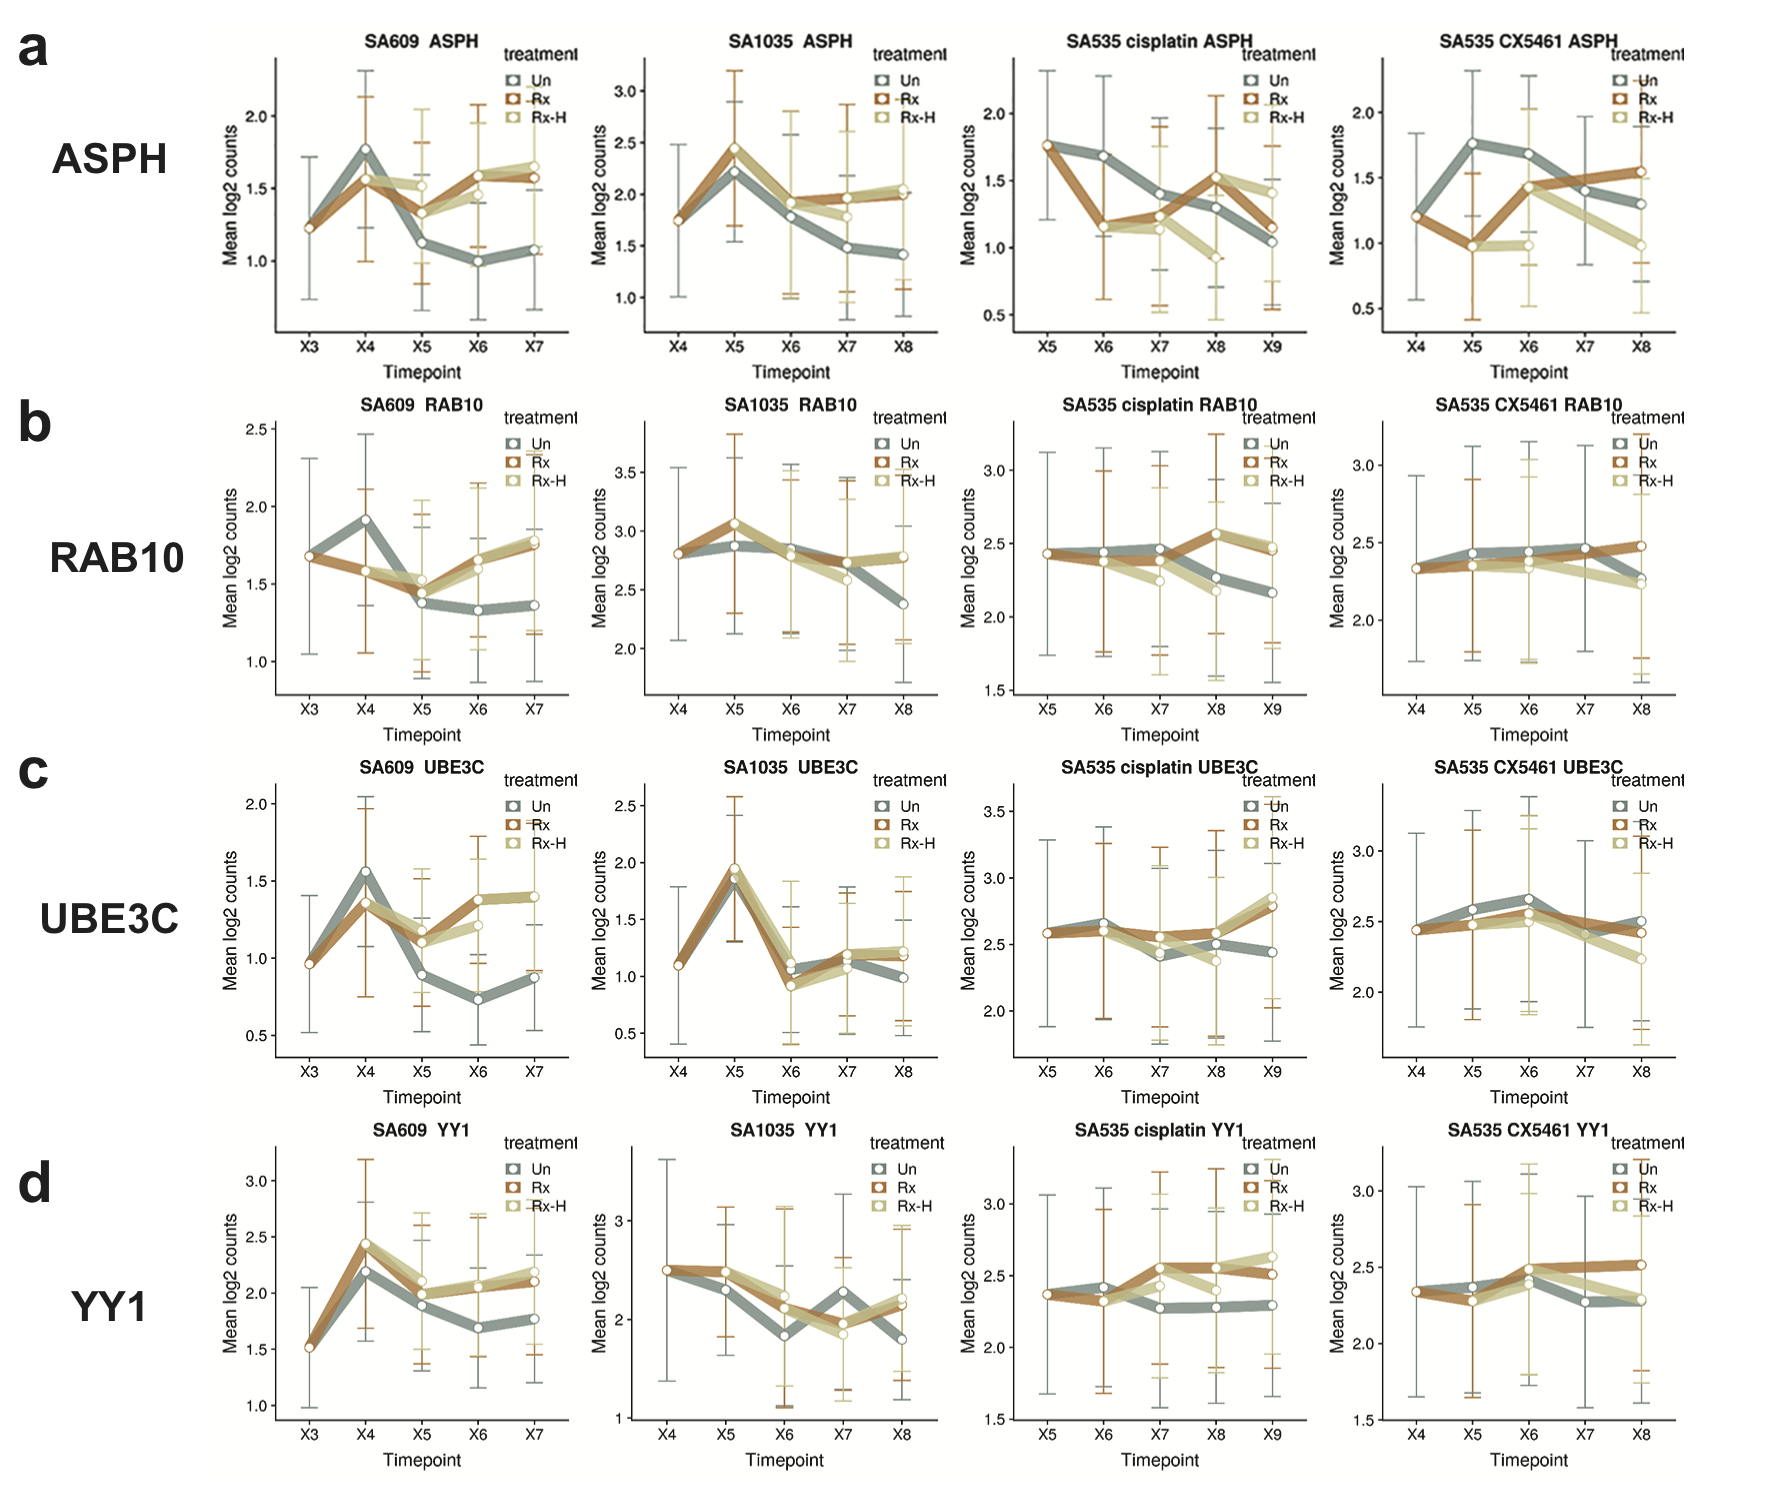
\includegraphics[width=\textwidth]{Figures/genelinetrajectories.pdf}
	
\caption[Gene expression changes over time]
	{\small
	 \textbf{Gene expression changes over time in all 4 TNBC PDX timseries} .
	}
	\label{fig:genelinetrajectories}
\end{figure}



\section{Discussion}

By using clonealign, we were able to assign single cell RNAseq to  DLP+ clones and we observed similar clonal proportion. UMAP suggested that the clones are behaving in relatively monomorphic way. From global survey of the copy number driven change in expression, \textit{in cis} proportion was found to be less as compared to the \textit{in trans} which is consistent with the mutation effects on expression. We know that cis-regulatory mutations are skewed toward decreased expression while trans-regulatory mutations are skewed toward increased expression \cite{metzger2016contrasting}.

The magnitude of individual gene expression differences between resistant and sensitive clones showed modest range of \textit{in cis} and \textit{in trans}. Although most of the genes are different but there are pathways that were common among the TNBC PDX models. 

SA1035 TNBC PDX behaves a little different as compared to the other two PDX models based on the activated pathways and proportion of individual gene expression \textit{in cis} and \textit{in trans}. This could be possibly explained based on the initial heterogeneity of this tumor. The DLP+ heatmap showed less heterogeneity as compared to SA609 and SA535 and the later was found to show the most heterogeneous tumor.

Some of the gene clusters were found to be increasing or decreasing along the time series of the PDX models but they require further detailed investigation at individual gene level to get enough evidence.






%\subsubsection{SA609-TNBC-FBI PDX up regulated pathways in resistant clone}


%\subsubsection{SA535-TNBC-BRCA deficient PDX up regulated pathways in resistant clone}
%Next we compared the emerging clone under drug pressure with the clone that could not survive the repeated drug exposures. We identified the following significantly up regulated pathways:
%- Apoptosis, Epithelial mesenchymal transition, Hypoxia, mitotic spindle, MTORC1 signaling, MYC targets-V1, P53 pathway, TGF Beta signaling, TNFA signalling via NFKB, UV response up, UV response down, KRAS signaling, Angiogenesis, PI3K AKT MTOR signaling, unfolded protein response.


%\subsubsection{SA1035-TNBC-APOBEC deficient PDX up regulated pathways in resistant clone}




%\subsection{key Pathways and genes shared among the three TNBC PDX}




%\subsection{Distinct genes monotonically increasing and decreasing with drug} 


